\documentclass[border=0.2cm]{standalone}

\usepackage{graphicx} %package to manage images
\graphicspath{ {./images} } 
\usepackage{tikz}
\usetikzlibrary{shapes.geometric}
\begin{document}

\begin{tikzpicture}

\node (rect) at (0,0) [draw,fill=black,,minimum width=2cm,minimum height=2cm] (rectangle)  {};

\node[trapezium,
    draw = black!80,
    text = black,
    align=center,
    fill = green!20,
    trapezium angle=80,
    minimum height=3cm,
    shape border rotate=270,
    left of = rectangle, node distance = 5cm ] (t1) { Encoder\\g\tiny e};  

\node[trapezium,
    draw = black!80,
    text = black,
    align=center,
    fill = blue!10,
    trapezium angle=80,
    minimum height=3cm,
    shape border rotate=90,
    right of = rectangle, node distance = 5cm ] (t2) { Decoder\\f\tiny e};    

\node[scale = .8, left of = t1, node distance = 7cm] (inputpic)  {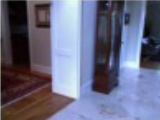
\includegraphics {input.png}};
\node[scale = .8, right of = t2, node distance = 7cm] (outputpic)  {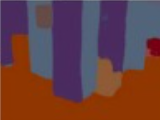
\includegraphics {images/output.png}};


\draw [-stealth] (t1.east) -- (rectangle.west) node[midway,right] {};
\draw [-stealth] (rectangle.east) -- (t2.west) node[midway,right] {};
\draw [-stealth] (inputpic.east) -- (t1.west) node[midway,right] {};
\draw [-stealth] (t2.east) -- (outputpic.west) node[midway,right] {};

\node[above of=rectangle, align=center, node distance=1.7cm] {Latent \\ Representation};
\node[above of=inputpic, align=center, node distance=1.7cm] {Input Image};
\node[above of=outputpic, align=center, node distance=1.7cm] {Output Map};
\node[below of=inputpic, align=center, node distance=1.7cm] {x};
\node[below of=outputpic, align=center, node distance=1.7cm] {y};

\end{tikzpicture}
 
\end{document}